\subsection{Resumen}
Esta implementación del filtro la vamos a utilizar para corroborar una de nuestras hipótesis planteadas. \\
El funcionamiento de esta implementación realizada en assembler es completamente diferente a la usada en SIMD. Además de diferente lo positivo de esta implementación es su simplicidad. \\
Lo malo de esta implementación es la cantidad de iteraciones a realizar y la cantidad de accesos a memoria por iteración.
El pseuocódigo es el siguiente:\\
//Tengo 6 registros temporales supongamos que se enumeran de R1...R6 todos de 1Byte\\
// El puntero a la imagen 1 lo voy a llamar Img1, el de la imagen dos Img2 y el puntero a la imagen de destino lo voy a llamar Dest\\
//Ademas de todos estos tengo un registro contador (Cont) que tiene como valor: Cont = ancho*alto que representa las iteraciones a rehalizar\\

while(Cont != 0){  	$~~~~~~~~~~$	//Itero tantas veces como píxeles tenga\\
$~~~~~~~~~~~$	R1$<$-$[$Img1$]$;  	$~~~~~~~~~~$	//traigo la componente red de la imagen 1\\
$~~~~~~~~~~~$	R2$<$-$[$Img2$]$; 	 $~~~~~~~~~~$	//traigo la componente red de la imagen 2\\
$~~~~~~~~~~~$	Img1++; 	 $~~~~~~~~~~$	//Me muevo un byte en la imagen 1\\
$~~~~~~~~~~~$	Imag2++; 	$~~~~~~~~~~$	//Me muevo un byte en la imagen 2\\
$~~~~~~~~~~~$	R3$<$-$[$Img1$]$ 	$~~~~~~~~~~$	//Traigo la componente Green de la imagen1\\
$~~~~~~~~~~~$	R4$<$-$[$Img2$]$ 	$~~~~~~~~~~$	//Traigo la componente Green de la imagen2\\
$~~~~~~~~~~~$	Img1++; 	$~~~~~~~~~~$	//Me muevo un byte en la imagen1\\
$~~~~~~~~~~~$	Img2++;        	$~~~~~~~~~~$	//Me muevo un byte en la imagen2\\
$~~~~~~~~~~~$	R5$<$-$[$Img1$]$; 		$~~~~~~~~~~$ //Traigo la componente Blue de la imagen1\\
$~~~~~~~~~~~$	R6$<$-$[$Img2$]$; 	$~~~~~~~~~~$	//Traigo la componente Blue de la imagen2\\
$~~~~~~~~~~~$	Img1+=2;	$~~~~~~~~~~$	//Apunto al siguiente pixel salteando la componente alpha\\
$~~~~~~~~~~~$	Img2+=2; 	$~~~~~~~~~~$	//Apunto al siguiente pixel salteando la componente alpha\\
$~~~~~~~~~~~$	//Ahora voy a calcular el modulo de la resta en cada uno de los componentes\\
$~~~~~~~~~~~$	R1$<$- mod(R1-R2)\\
$~~~~~~~~~~~$	R2$<$-mod(R3-R4)\\
$~~~~~~~~~~~$	R3$<$-mod(R5-R6)\\
$~~~~~~~~~~~$	//una vez que tengo  en R1, R2, R3 el modulo de las restas de cada uno de los componentes paso a calular el maximo entre esos 3\\
$~~~~~~~~~~~$	R1$<$- max(R1, R2); \\
$~~~~~~~~~~~$	R1$<$-max(R1, R3);\\
$~~~~~~~~~~~$	//Finalmente los muevo a la imagen de destino cuidando de poner 255 en la componente alpha\\
$~~~~~~~~~~~$	$[$Dest$]$$<$-R1;\\
$~~~~~~~~~~~$	Dest++;\\
$~~~~~~~~~~~$	$[$Dest$]$$<$-R1;\\
$~~~~~~~~~~~$	Dest++;\\
$~~~~~~~~~~~$	$[$Dest$]$$<$-R1;\\
$~~~~~~~~~~~$	Dest++;\\
$~~~~~~~~~~~$	$[$Dest$]$$<$-255; 	$~~~~~~~~~~$	//muevo el 255 en byte obviamente\\
$~~~~~~~~~~~$	Dest++;\\
$~~~~~~~~~~~$	Cont--;\\

}

\subsection{Assembler con SIMD es más rápido que la Assemler sin SIMD}

¿Es esta hipótesis verdadera? La respuesta es sí. Pero... ¿por qué?. \\
Primero voy a hacer varios casos de prueba entre ambas implementaciones para analizar su comportamiento. Lo esperado a observar en esta comparación es una notable diferencia a favor del filtro realizado usando SIMD.\\
¿Y como medimos esta diferencia?\\
 La métrica decidida para esta y para otras comparaciónes es la métrica dada por los Ticks del reloj.\\
 Para eso voy a realizar varios casos de prueba y voy a comparar la cantidad de ciclos de clock utilizados .\\

 \subsection{Gráficos SIMD vs sin SIMD}



 \begin{figure}[H]
\begin{center}
%\minipage{0.8\textwidth}
  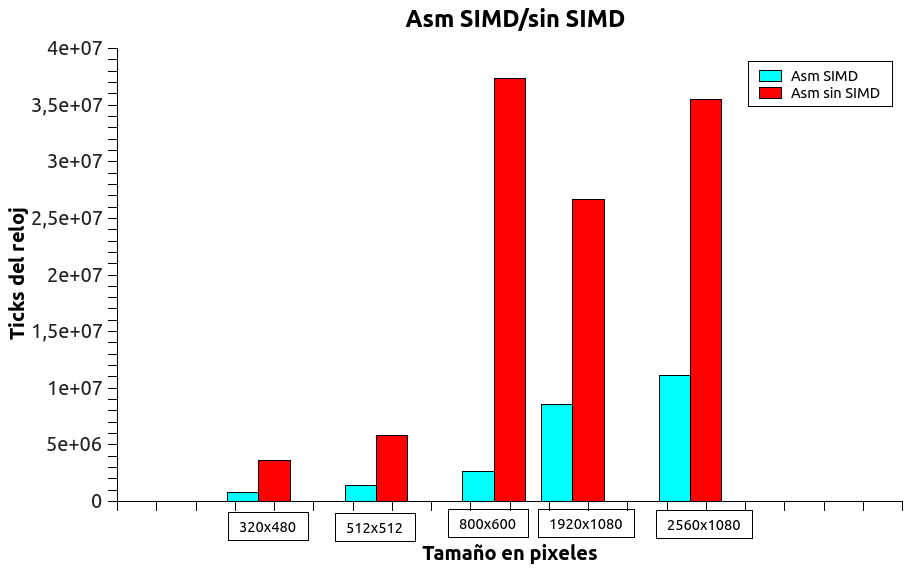
\includegraphics[width=\linewidth]{diffsinsimd/simdSinSIMD.png}
  %\endminipage
\end{center}
\end{figure}

 Como esperabamos, el uso del modelo SIMD es muy superior ya que tiene menor cantidad de iteraciones, menor acceso a memoria por iteración y mayor capacidad de pocesamiento. No hay necesidad de examinarlo mas a fondo ya que hoy en día casi se puede realizar una demostración formal sobre la ventaja de SIMD sobre asm sin usar SIMD\\
\subsection{La implementación en C es más rápida que la implementación en Assemler sin SIMD}
 A continuación vamos a comparar el rendimiento entre ĺa implementación del filtro en c y su implementación en assembler sin el uso de SIMD.\\
 Nuestra hipótesis consiste en que la implementación en C es más rápida que la implementación realizada en Assembler. Para tratar de corroborar esto vamos primero a comparar el tiempo en Ticks del reloj utilizados para procesar una imagen en ambas implementaciones.  Lo esperado en este caso es que el filtro en C demore menos. \\ 
 El siguiente gráfico muestra, para varias imagenes de distinto tamaño, el tiempo de proceso dado en ticks de reloj de la implementación en C comparado a la implementación en Assembler sin SIMD. \\

 \subsection{Gráficos C vs sin SIMD}

 \begin{figure}[H]
\begin{center}
%\minipage{0.8\textwidth}
  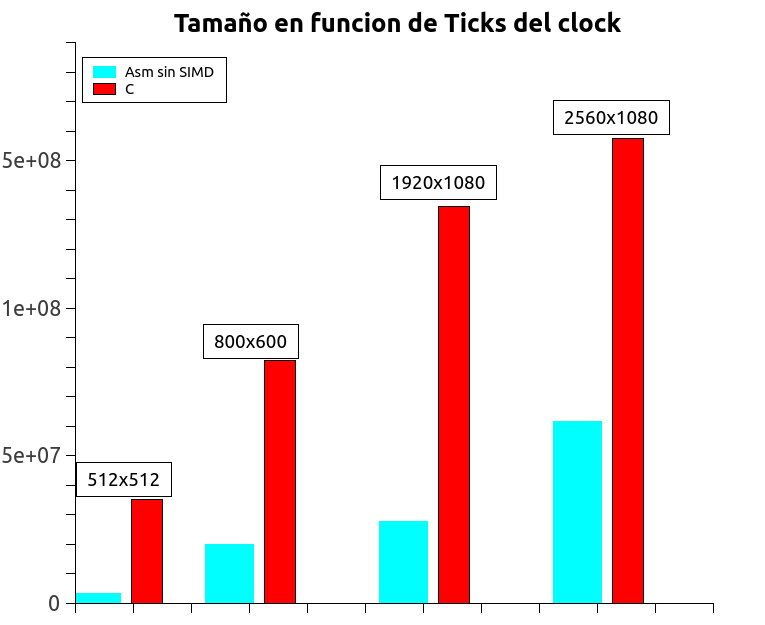
\includegraphics[width=\linewidth]{diffsinsimd/ASMssdC.png}
  %\endminipage
\end{center}
\end{figure}
El gráfico anterior muestra, a diferencia de lo supuesto anteriormente, un menor tiempo de procesamiento para el filtro implementado assembler sin SIMD.\\
¿Y por qué sucede esto?\\
La diferencia consiste principalmente en que en la implementación de Assembler no hago accesos innecesarios a memoria. Es decir, en cada ciclo accedo en total nueve veces a memoria, ni mas ni menos.\\
 Uno estaría tentado a decir que sucede lo mismo en la implementación del filtro en C, estaría tentado a decir que también accedo esa misma cantidad de veces a memoria pero a diferencia de la implementación en Assembler, accedo más veces indirectamente porque en mi función tengo variables y las variables se guardan en el Stack.\\
 En mi implementación en C de la función diff tengo varias variables y opero con ellas en todo momento ya sea para hacer una resta, para calcular un maximo entre gamas o también incluso para guardar mi resultado en la imagen de destino. Cada una de estas operaciones realizadas con las variables demanda un acceso a memoria, mas específicamente al stack, para poder obtener su valor dando como resultado una mayor cantidad de accesos a memoria y una mayor cantidad de Ticks del reloj en cada iteración del ciclo. Por ende concluimos que nuestra hipótesis resultó ser falsa\\
 

  
 





